\section{Wind Turbine Power Model}
    
Power is defined as the change of energy over time. It describes how much energy is transferred or used over a period of time. With this, power can be describe as
\begin{equation}
    P = \frac{dE}{dt}
\end{equation}
where $P$ is power $\frac{dE}{dt}$ is the change of Energy over the change of time. Since the Wind turbine uses Kinetic energy to convert into power, using the Kinetic Energy equation,
\begin{equation}
    E = \frac{1}{2}mv^{2}
\end{equation}
where $E$ is the Kinetic energy, $v$ is the velocity of the wind and $m$ is the mass of the wind. The power can of the wind can now be expressed as
\begin{equation}
    P = \frac{dE}{dt} = \frac{1}{2}v^{2}\frac{dm}{dt}
\end{equation}
where $\frac{dm}{dt}$ is the mass flow rate. The velocity of the wind is assumed to remain constant over a period of time, and the mass of the wind changes depending on the displacement of the wind through the rotor area.

The mass flow rate can be defined as
\begin{equation}
    \frac{dm}{dt} = \rho A\frac{dx}{dt}
\end{equation}
where $A$ is the area of the wind at the wind turbine, $\rho$ is the wind density and $\frac{dx}{dt}$ is distance over time or the velocity $v$ of the wind. Since $A$ is the area where the wind is occupying at the wind turbine, $A$ is the total area where the rotor spans while spinning (rotor area). Using this equation, the power of the wind turbine is now
\begin{equation}
    P = \frac{1}{2}v^{2}\frac{dm}{dt} = \frac{1}{2}v^{3}\rho A
\end{equation}
Note that the wind turbine cannot absorb all the power from the wind. In fact, the Power Coefficient $C_p$ determines how much Kinetic Energy from the wind that can be converted into mechanical energy at maximum. There is a percentage of energy lost from the wind when the wind turbine is operating. Thus, the Power of wind turbine is
\begin{equation}
    P =  \frac{1}{2}v^{3}\rho A C_{p}
\end{equation}

Using the specifications of the wind turbine with $40m$ rotor diameter along with the normal air density $\rho = 1.225kg/m^{3}$ and standard average power coefficient of $C_{p}=0.4$, the power ($kW$) of the wind turbine used in this experiment is 
\begin{align*}
    P &=  \frac{1}{2}v^{3}(1.225kg/m^3)(\pi (20m)^2)(0.4)\\
        &= 307.87v^{3} &(in \;Watts) \\
        &= 0.3v^3 &(in \;kiloWatts)
\end{align*}



\section{Wind Farm Model}
    The wind farm is modelled in such a way that there would only be a limited number of turbines on the wind farm. Abdelsalam et al. \cite{this} used the same model as with Mosetti et al. \cite{windturbine5} where a wind farm with dimensions $K meters$ by $K meters$ is modelled as a $\frac{K}{200\;m}$ by $\frac{K}{200\;m}$ matrix where each cell maps to a land area of $200m$ by $200m$ in which the wind turbine sits in the middle. This means that an $n$ by $n$ matrix model maps to a $200n$ $meters$ by $200n$ $meters$ wind farm, see Figure \ref{windFarmModel}. For example, a wind farm with dimensions of $1km$ by $1km$ shall have a matrix model of size of
    \begin{equation}
        1km\;by\;1km\Rightarrow 1000m\;by\;1000m\Rightarrow 0.005(1000m)/m\;by\;0.005(1000m)/m\Rightarrow 5\;by\;5
    \end{equation}
    In the same way as a $5\;by\;5$ matrix model maps to a wind farm with dimensions
    \begin{equation}
        5\;by\;5\Rightarrow 200(5)\;meters\;by\;200(5)\;meters\Rightarrow 1000m\;by\;1000m
    \end{equation}
    Note that a cell in the matrix model can accommodate only one wind turbine. Therefore for an $n$ by $n$ matrix model of the wind farm, the number of slots for the wind turbines in the wind farm is $n^2$, and the number of turbines $N$ possible for the wind farm is
    \begin{equation}
        1\leq N\leq n^2-1
    \end{equation}
    The number of wind turbines cannot be $N=1$ or $N=n^2$ because the optimization will no longer have sense.
    %how to label the positions of each turbine on the wind farm
    
    \begin{figure}[h]
        \centering
        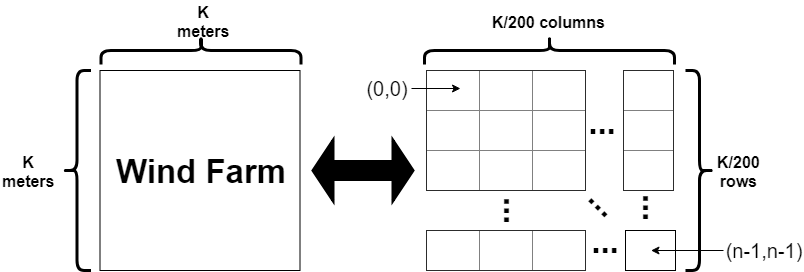
\includegraphics[width=\linewidth]{Figures/windFarmModel.png}
        \caption{Matrix model of a wind farm showing the possible locations of wind turbines}
        \label{windFarmModel}
    \end{figure}
    
    A location in the wind farm or a cell in the matrix model is labelled as a combination of row number and column number. As shown in Figure \ref{windFarmModel}, the location on the top leftmost of the matrix is labelled as $(0,0)$ which means row number 0 and column number 0, and the bottom rightmost location is labelled as $(n-1,n-1)$ which means row number $n-1$ and column number $n-1$.
    
    \begin{figure}[h]
        \centering
        
\includegraphics[width=100mm]{Figures/windDirection.png}
        \caption{Wind direction on the wind farm measured in degrees}
        \label{windDirection}
    \end{figure}
    
    %angles of entry of the wind
    The angle of the wind direction is measured as how many degrees is the source of wind away, in a counterclockwise manner, from the north of the wind farm. From Figure \ref{windDirection}, a wind direction of $\theta=0^\circ$ means the wind blows from the north, a wind direction of $\theta=45^\circ$ means the wind blows from the northwest, a wind direction of $\theta=90^\circ$ means the wind blows from the west, and so on.
    
    %how the wind enters the rotor and how the wind disperses
            
\section{Wake Model}
    Siting a wind farm must consider several factors to consider to maximize the output energy while minimizing the total cost. Several wind qualities are taken into consideration including, average wind velocity, frequency of wind, time when the wind blows, etc. Not only the wind quality, also the location must be examined. Generally, the higher the altitude of the terrain, the faster the general wind speed is. This is ideal for greater return and when to break even when investing on wind farms. Though faster wind is ideal, too fast would prove to be more costly. If the wind site is stormed quiet frequently, it might damage the wind turbines causing more money for maintenance. Wind turbines also stops when the wind is too strong causing them to not produce energy. After finding the site, the availability and legality of the site is then looked into. This includes environmental concerns in both air and terrain. Aviation concerns includes if the site is a main path for birds or airplanes. Terrain includes surrounding ecosystems or communities \cite{book1}.
    
    On a wind farm, when the wind blows on multiple rows of wind turbines, the wind through the downstream wind turbine is always slower than the wind through the upstream wind turbine. This event is called the \textbf{wake effect}. The velocity of the wind is reduced when it runs through the blades of the wind turbine. Then this wake will run through another wind turbine which will have an even slower velocity. This forms a chain reaction which each wind turbine. Since the input energy is exponentially lower with each wind turbines, the total output will give diminishing returns in proportion to the total cost of a wind turbine \cite{wakelosses}. This is usually caused by non-optimal positioning of the wind turbines and will affect overall produced energy for that particular wind site.

    %JENSENS'S WAKE MODEL
    Jensen \cite{book2} proposed a model for single wake interaction of wind turbines. The \textbf{Jensen's Wake Model} is a simple model used to accurately calculate the wake of the wind. The wake model is given by
        \begin{equation}
            u = u_{\infty}\left[1 - 2a\left(\frac{r_{0}}{r_{0}+\beta x}\right)\right]
            \label{jensen}
        \end{equation}
    where $u$ is the downstream wind speed due to wake of upstream wind turbine, $u_{\infty}$ is the undistributed inflow speed, $a$ is axial induction factor, $\beta$ is the entrainment constant, $r_{0}$ is the radius of the rotor and $x$ is the directed distance parallel to the direction of the wind from the upstream wind turbine to the downstream wind turbine \cite{thrust}. Note that the upstream turbine is the turbine that provides the wind to the downstream turbines. Which means that the wind from a wind turbine that hits subsequent wind turbines is called the upstream wind and the resulting wind from the subsequent wind turbines is the downstream wind. Undistributed inflow speed meaning that all affected upstream turbines from the initial wind will receive the same amount of wind speed and not divided among them.
    
    The Jensen's Wake model was derived if the assumption that the near field, which is the vibration of the wind turbine because of the mechanism, is ignored then the momentum equation:
        \begin{equation}
            \pi r_{o}^{2} v_{o} + \pi (r^{2} - r_{o}^{2})u_{\infty} = \pi r^{2} v
        \end{equation}
    where $v_{o}$ is the velocity behind the rotors, $r_{o}$ is the rotor radius, $r$ is the resulting radius at distance $x$, $u_{\infty}$ is the undistributed inflow speed, and $v$ is the resulting speed at a specific distance $x$. The $r$ can be expressed as $r_{o} + \alpha x$, where $\alpha$ is the entrainment constant and $x$ is the downstream distance of the wind. This is assumed because $r$ is  proportional to the distance $x$ which means that the farther the wake travel from the wind turbine at $x$ the larger the area of the wake is at radius $r$. Note that the Area of a circle is used for the momentum because the wind turbine's rotor is circular thus swirling the initial wind to create the wake tunnel. Solving for v and assuming that the velocity of the inflow wind just behind the rotor is $\frac{1}{3} u$, the model is formed where $v = u$ \cite{book2}.
        \begin{figure}
            \centering
            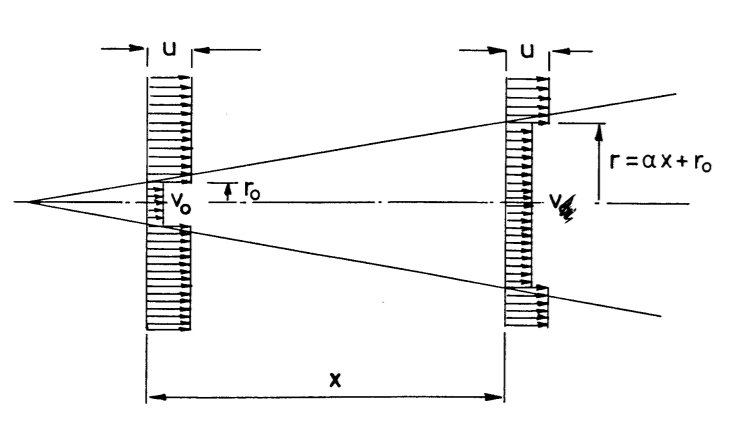
\includegraphics{Figures/wakemodeJensen.PNG}
            \caption{The visual representation of the Wake model\cite{book2}}
            \label{fig:my_label}
        \end{figure}
    
    Thrust Coefficient describes the device's maximum thrust force. Since the wind decelerates when it is being used by an energy-extracting devices, thrust coefficient is used to know how much energy is lost from converting the kinetic energy of the wind to mechanical energy of the devices. Knowing the Thrust Coefficient, $C_{T}$, given as
        \begin{equation}
            C_{T} = [4a(1-a)]
        \end{equation}
    the Axial induction Factor, $a$, is derived from the Thrust Coefficient and used to the model, where a is
        \begin{equation}
             a = 0.5 -0.5\sqrt{1-C_{T}}
        \end{equation}
    The wind's velocity when passing through the wind turbine is always lowered. This is due the the some of the wind in axial momentum hitting the turbine will be deflected back, thus slowing the upstream velocity. The fractional loss of wind speed after being worked on by the wind turbine to the initial wind speed is measured as the Axial Induction Factor\cite{thrust}.
    
    The Entrainment Constant, $\beta$, is then calculated as
        \begin{equation}
            \beta = \frac{0.5}{ln(z/z_{0})}
        \end{equation}
    where $z$ is the hub height and $z_{0}$ is the surface roughness \cite{book2, thrust}. Entrainment, by definition, comes from the word entrain, which means a substance that is entrap inside another substance. In this case, the wind turbine inside the wind. Hub Height is the wind turbine's height above ground which is the distance between the center of the rotor to the surface ground while the surface roughness is the measured roughness of the ground.
    
    However, Abdelsalam et al. \cite{this} also used a simple modification of Jensen's Wake Model used by Mosetti et al. \cite{windturbine5}, Grady et al. \cite{windturbine3} and Emami et al. \cite{windturbine6} given by
    \begin{equation}
        u = u_{\infty}\left[1 - 2a\left(\frac{r_{1}}{r_{1}+\beta x}\right)^2\right]
        \label{jensen}
    \end{equation}
    where
    \begin{equation}
        r_1=r_o\sqrt{\frac{1-a}{1-2a}}
    \end{equation}
    
        \begin{figure}[h]
            \centering
            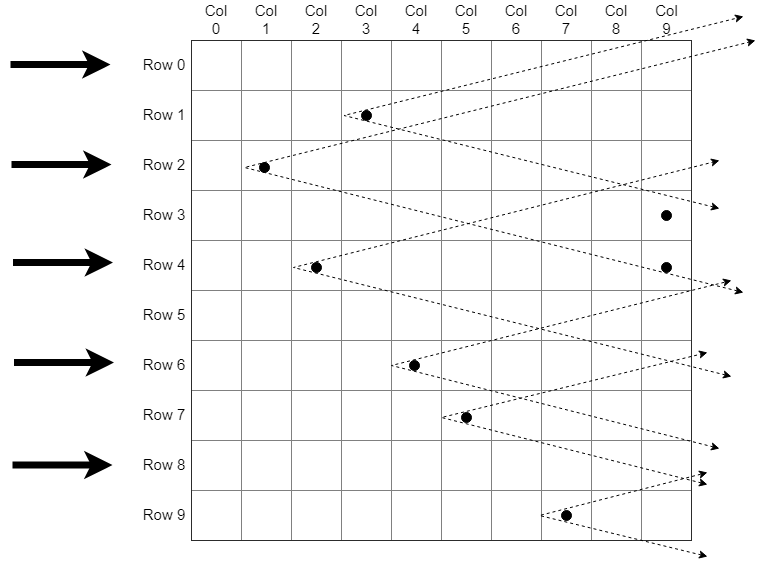
\includegraphics[width=\linewidth]{./Figures/multWake.png}
            \caption{Multiple Wake Interaction \cite{wakemodel}}
            \label{multWake}
        \end{figure}
        
    Unfortunately, it is not always the case that there is only a single wake downstream. Most of the time, the wind turbine downstream is in wake of a number of wind turbines upstream which are also in wake of another wind turbines upstream called \textbf{multiple wake interaction}. As shown in Figure \ref{multWake}, turbines at location $(3,9)$ and $(4,9)$ are both under the wakes of turbines located at $(2,1)$ and at $(4,2)$. For the case of multiple wake interaction, Abdelsalam et al. \cite{this} used the sum of squares method to individually compute the wind speed at each turbine during multiple wake interaction. The \textbf{Sum of Squares}, in statistics, is a measure of deviation of data points from the mean. In this case, the sum of squares is modelled as
        \begin{equation}
            \left(1-\frac{u_i}{u_\infty}\right)^2=\sum_{j=1}^{n}\left(1-\frac{u_{ij}}{u_j}\right)^2
        \end{equation}
    where $u_i$ is the wind speed at the $i^{th}$ wind turbine (downstream) from the list of all the turbines, $u_\infty$ is the undistributed wind inflow, $u_{ij}$ is the expected wind speed at the $i^{th}$ turbine due to the single wake interaction of the $j^{th}$ turbine (upstream), and $u_j$ is the wind speed at the $j^{th}$ wind turbine. Note that if a downstream wind turbine only experiences a single wake interaction then the modified Jensen's model is used, and since $u_{ij}$ is a wind speed due to a single wake interaction, it is also computed using the modified Jensen's model.
    
    \begin{figure}[h]
        \centering
        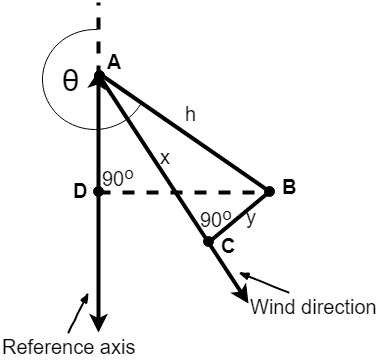
\includegraphics[width=100mm]{Figures/comp1.png}
        \caption{Diagram of two wind turbines showing the distance between them parallel to the wind direction}
        \label{comp1}
    \end{figure}
    
    To be able to determine if a wind turbine is under the wake of an upstream turbine, the first thing to do is to find the directed distance parallel to the wind direction between two wind turbines because the wake model $u$ is a function of that distance or $x$. From Figure \ref{fig:my_label}, it is shown that the resulting radius of the wind coming from the upstream wind turbine is computed as
    \begin{equation} \label{rValue}
        r=ax+r_0
    \end{equation}
    which means that a wind turbine is influenced by the wake of an upstream wind turbine if its directed distance from the line parallel to the wind direction and the passes through the center of the upstream turbine is less than the resulting radius of the wind coming from the upstream turbine $r$.
    
    From our model of the wind farm where the turbine locations are coordinates in the matrix, let $(i_0,j_0)$ be the location of the upstream turbine and $(i_f,j_f)$ be the location of the candidate downstream wind turbine. For wind directions greater than or equal to $0^o$ and wind directions less than $90^o$, let the vertical line passing through the center of the upstream wind turbine be the reference axis and from Figure \ref{comp1}, points are labelled as $A$, $B$, $C$ and $D$ where points $A$ and $B$ are the centers of the upstream wind turbine and the candidate downstream wind turbine respectively. Triangle $ADB$ forms a right angle at angle $ADB$ where the sides can be expressed as
    \begin{equation}
        \overline{AD} = \left| i_f-i_0 \right|
    \end{equation}
    \begin{equation}
        \overline{DB} = \left| j_f-j_0 \right|
    \end{equation}
    and by the Pythagorean Theorem, the hypotenuse $\overline{AB}$ is expressed as
    \begin{equation}
        h=\overline{AB} = \sqrt{\overline{AD}^2+\overline{DB}^2}=
                        \sqrt{\left| i_f-i_0 \right|^2+\left| j_f-j_0 \right|^2}
    \end{equation}
    It follows that from the same triangle in the figure, angle $BAD$ shall have magnitude of
    \begin{equation}
        \angle BAD = tan^{-1}\left| \frac{\overline{DB}}{\overline{AD}} \right|
                    = tan^{-1}\left| \frac{\left| j_f-j_0 \right|}{\left| i_f-i_0 \right|} \right|;
                    \;\;\; 0^o\leq\theta<90^o\cup180^o\leq\theta<270
    \end{equation}
    and angle $CAB$ shall be
    \begin{equation}
        \angle CAB = \left( \theta \;mod\; 90^o \right)-\angle BAD
                    = \left( \theta \;mod\; 90^o \right)-tan^{-1}\left| \frac{\left| j_f-j_0 \right|}{\left| i_f-i_0 \right|} \right|
    \end{equation}
    From the triangle $ACB$, the sides $x$ and $y$ are derived as shown below.
    \begin{equation} \label{x1}
        x=h\cdot cos\left( \angle CAB \right)=\left(\sqrt{\left| i_f-i_0 \right|^2+\left| j_f-j_0 \right|^2}\right)cos\left( \left( \theta \;mod\; 90^o \right)-tan^{-1}\left| \frac{\left| j_f-j_0 \right|}{\left| i_f-i_0 \right|} \right| \right)
    \end{equation}
    \begin{equation}\label{yValue}
        y = \sqrt{h^2-x^2}
    \end{equation}
    
    Luckily, the formula above for $x$ and $y$ works for any wind directions less than $360^o$ and except $\theta=90^o$ and $\theta=270^o$. For wind directions $\theta=90^o$ and $\theta=270^o$, the concept only works if the expression $\theta \;mod\; 90^o$ from equation \ref{x1} stays $90^o$.
    Hence, the formula for $x$ for all wind directions is
    \begin{equation} \label{finalX}
        x =
        \begin{cases} 
            \left(\sqrt{\left| i_f-i_0 \right|^2+\left| j_f-j_0 \right|^2}\right)cos\left(90^o-tan^{-1}\left| \frac{\left| j_f-j_0 \right|}{\left| i_f-i_0 \right|} \right| \right) & \theta \neq 90^o \;AND\; \theta \neq 270^o \\
            \left(\sqrt{\left| i_f-i_0 \right|^2+\left| j_f-j_0 \right|^2}\right)cos\left( \left( \theta \;mod\; 90^o \right)-tan^{-1}\left| \frac{\left| j_f-j_0 \right|}{\left| i_f-i_0 \right|} \right| \right) & elsewhere
        \end{cases}
    \end{equation}
    
    A wind turbine located at $(i_o,j_0)$ is downstream of an upstream wind turbine located at $(i_f,j_f)$ if $y$ from equation \ref{yValue} is less than or equal the resulting radius of the downstream wind $r$ from equation \ref{rValue}.
    
    